\chapter{Characteristics and constraints of rehabilitation exergames}
\label{ch:characterising}

To develop a \ac{PX} evaluation model for rehabilitation exergames, we should understand what a rehabilitation exergame represents and how to characterise it for evaluation purposes considering its therapeutic purpose. In this section, we propose a definition of rehabilitation exergames considering that those are exergames, have therapeutic purposes and are used within rehabilitation therapies. Then, we present a set of constraints to consider when evaluating this kind of exergames. Finally, we propose an approach to characterise rehabilitation exergames for evaluation purposes based on the proposed definition and constraints.

%-----------------------------------
\section{Defining rehabilitation exergames} % Definition --------------------------
\label{sec:def_reh_ex}
Rehabilitation exergames should be defined considering their nature as exergames, their therapeutic purposes and their use as part of rehabilitation therapies. Below, we study those three aspects and propose a definition for rehabilitation exergames.

\subsection{Exergames}
\label{sub:def_ex}
% Definition
According to \textcite{Mueller2011}, an exergame is a game that employs body movement to enable player's interaction; i.e., the outcome of the game is determined by the player's physical effort. Also, \textcite{Pirovano2016} defines an exergame as a game built into an exercise structure. This definition implies that the associated exercises should guide the whole game design process. It may be important for rehabilitation exergames since exercises are directly related to their therapeutic purpose. Furthermore, \textcite{Sinclair2009}, defines an exergame as a merger of a digital game with exercise equipment, emphasising the role that the interaction devices play in the experience of playing exergames.

\subsubsection{Exergames Models}
\label{subsub:eg_models}
Exergame models allow achieving a comprehensive understanding of what the exergame concept may comprise. Below, we outline three of these models:

\begin{enumerate}
    \item \emph{The Four Lenses Model}: \textcite{Mueller2011} propose an exertion framework as an attempt to describe how exergames can use technology to create more compelling exergames. This framework is based on the four lenses, as they call them, and is centred on the player's body to understand the interaction. The four lenses allow considering the body in a structured way when designing an exergame.
    
    The first lens is \emph{The Responding Body}, which concerns with the internal body reactions before, during and after physical activity. The responding body impacts the design process since it affects interaction; i.e., when a player becomes fatigued or stronger as a consequence of exercise. Thus, the game challenge should adapt to player needs and skills, by controlling or monitoring responding body using physiological methods such as \ac{HR} or \ac{EEG}.
    
    The second lens is \emph{The Moving Body}, which corresponds to the re-positioning of the player's body parts during physical activity. Intensity, continuity and variety of the movement can enrich the game experience by providing resources and constraints to the exercise involved in a game.
    
    The third lens is \emph{The Sensing Body}, which describes how the player's body senses and experiences the world, including physical and virtual objects involved in a game exercise. Considering the sensing body during design may allow designers to achieve a richer game experience in a hybrid space
    
    The fourth lens is \emph{The Relating Body}, which encompasses how players relate to other people and technology. Adding a social layer to a game is key for people to participate in physical activity.
    
    Additionally, \textcite{Mueller2011} highlight some characteristics of exergames. First, uncertainty is desirable since it contributes to offering suspense and surprise along the experience. Particularly, game designers should consider that player's exercising brings a degree of uncertainty since his/her body movements are unpredictable.  Thus, they should manage the relationship between the programmed uncertainty and the uncertainty arising from the player's exercise. Second, movement awareness contributes to \ac{PX} when exercising. Increasing movement awareness of players; e.g., by providing feedback about energy expenditure; may foster competition among them. While decreasing such awareness will distract the player from discomfort caused by exercising. Third, the player's expression of exertion may arise naturally as in sports. Although such expression does not allow a player to progress along the game, it contributes positively towards \ac{PX}. An exergame may support expression by highlighting players responding body characteristics. Fourth, adding rhythm to the game exertion can benefit aspects such as motor skills acquisition and discomfort dissociation. Fifth, designers should consider that exertion has an associated risk of injuring players in order to avoid a negative \ac{PX}. Finally, exergames have to assist players in understanding the associated exertion. It will enable players to play consciously and safety; e.g., knowing \ac{HR} while jogging allows a player to plan future activity. By mapping physical movements to a virtual world meaningfully is key to support exertion knowledge.
    
    \item \emph{\ac{ISCAL} Model}: \textcite{Zhang2011} proposed this model to build a Virtual Network Marathon. The model is based on five constructs: immersion, scientificalness, competitiveness, adaptability and learning. Immersion is the subjective impression of participating in a "realistic" exercise experience. Meanwhile, scientificalness means to perform exercise effectively and to avoid over-exercise; e.g., by including warming up and cool down stages before and after the exercise. Moreover, competitiveness enables players to satisfy their need of “getting better” at something. Adaptability refers to adjusting the game difficulty dynamically according to each player's needs. Finally, learning refers to offering players the opportunity to learn something while participating in the physical activity. \citeauthor{Zhang2011} argue that an exergame should support all constructs in order to provide an engaging experience.
    
    \item \emph{Dual Flow Model}: \textcite{Sinclair2007} propose this model due to the two purposes of an exergame: exercising and entertaining. The model comprises two constructs: attractiveness and effectiveness. Attractiveness motivates players to play and to continue playing in the future. It is closely related to fun and may be achieved by offering a balance between game challenges and player skills. That is, maintaining players in the flow zone \autocite{flow}.
    Effectiveness relates to the exercise involved in a game. An effective exergame has to result in health benefits for players, including fitness or rehabilitation. \citeauthor{Sinclair2007} propose a flow zone associated with the exercise involved in the game. In this case, an exergame has to provide a balance between the intensity of the exercise and the player's skills to perform the said exercise. A physiologically imbalanced exergame results in failure, deterioration or no-benefit for players. To achieve balance, an exergame has to collect feedback form player about fatigue, exercise level and boredom to adjust the challenge level accordingly.
\end{enumerate}

\subsection{Therapeutic games}
\label{sub:def_therapeutic_g}
A therapeutic game provides a cognitive or motor training to improve patient's health condition \autocite{Mader2012}. Specifically, a therapeutic exergame has to support the primary and secondary goals of exercises. Primary goals correspond to the movements involved in an exergame. Those are achieved by mapping desired movements into gameplay mechanics.  Meanwhile, secondary goals refer to the correctness with which patients perform the expected physical exercises \autocite{Pirovano2016}. Thus, secondary goals differentiate therapeutic exergames form normal exergames, and movement correctness should be ensured when using exergames for therapeutic purposes.

\subsection{Rehabilitation therapy}
\label{sub:def_rehab_therapy}
Rehabilitation aims to enable people with disabilities to participate in daily life activities by improving their health status \autocite{Wiemeyer2015}. To regain lost functions, patients must execute repetitive movements correctly \autocite{PirovanoAdvisor2012}. A typical therapy session includes the following tasks and activities:

\begin{enumerate}
    \item \emph{Configuration and Personalisation}: physiotherapists select correct exercises, establish therapy goals according to patients’ initial diagnosis and schedule therapy sessions.
    \item \emph{Supervision}: includes \textit{monitoring} correct execution of movements, \textit{providing immediate feedback} to guide patients along therapy sessions, \textit{adapting} patient’s movements and postures according to his/her performance, \textit{extracting physiological and motion data} and \textit{motivating} patients to complete their therapy.
    \item \emph{Assessment}: physiotherapists should use gathered to \textit{assess} obtained results and \textit{adapt} therapies according to patient’s progress.
\end{enumerate}

Therefore, we define a rehabilitation exergame as follows:\\

\emph{A rehabilitation exergame is a therapeutic exergame that assists rehabilitation therapies in one or more tasks.}

%-----------------------------------
\section{Materials and methods} % Materials -----------------------------------
\label{sec:mats_mets_char}
% Interviews (Include leading questions), observation, (/)
% Thematic content analysis (for qualitative research) using affinity charts (/)
% One coder (/)
% Validation: Review by physiotherapists (/)
\subsection{Participants}
We conducted five semi-structured interviews along two sessions. Two physiotherapists participated in both sessions, while a third physiotherapist joined the second session. All physiotherapists belong to the Evaristo Garc\'ia University Hospital in Cali Colombia. The goal of the first session was to characterise the context in which rehabilitation exergames are employed. We aimed to identify possible constraints that might limit the evaluation of \ac{PX} for this kind of games. We guided the interview of the first session using the following questions:

\begin{enumerate}
    \item What kind of patients participate in physical therapies?
    \item How is the patients' motivation towards physical therapies?
    \item What factors affect patients' motivation towards physical therapies?
    \item What activities occur during physical therapy sessions?
    \item Who participates in physical therapy sessions?
    \item How long does a therapy session takes?
    \item What information is collected during therapy sessions?
    \item How is patients' progress tracked?
\end{enumerate}

The goal of the second session of interviews was to identify physiotherapists expectations and requirements regarding the use of rehabilitation exergames. One of the physiotherapists had been collaborating in the development of a collection of rehabilitation exergames. The second interviews were conducted using the following questions.

\begin{enumerate}
    \item Who can decide if a patient can use a rehabilitation exergame as part of his/her therapies?
    \item How can a rehabilitation exergame be used as part of a physical therapy?
    \item When can a rehabilitation exergame be used as part of a physical therapy?
    \item How do you expect to use rehabilitation exergames?
    \item How do you expect that rehabilitation exergames assist patients?
\end{enumerate}

Both interviews were recorded. We analysed the collected data using the thematic content analysis method \autocite{Burnard2008}. We transcribed all interviews to produce a list of relevant statements. The selected statements were closely related to one or more of the mentioned questions. Then, we assigned a theme to each statement to produce our initial coding framework. After that, we grouped themes to reduce the number of categories. We continued until we obtained four categories for our final coding framework. The final coding framework was shared with one of the physiotherapists to validate that our results represented participants views. The physiotherapist clarified or added information to five statements, this validation did not affect the resulting categories. The conducted study is illustrated in \autoref{fig:constraintsIdentification}.

\begin{figure}[htb]
\myfloatalign
{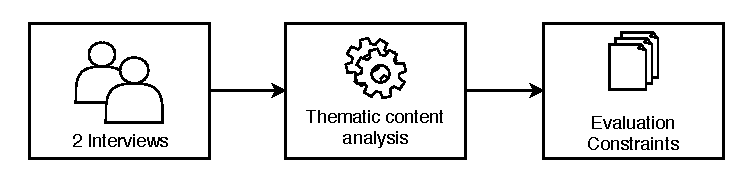
\includegraphics[width=\linewidth]{gfx/characterisation/constraintsIdentification}} \quad
\caption{Evaluation constraints identification process}\label{fig:constraintsIdentification}
\end{figure}

%-----------------------------------
\section{Findings} % Findings -----------------------------------
\label{sec:findings_char}
%-----------------------------------
\subsection{Constraints of evaluating PX in rehabilitation exergames} % Constraints -----------------------------------
\label{sec:constraints}

Rehabilitation exergames have constraints that evaluators should consider to perform a relevant PX evaluation. Otherwise, the occurrence or completion of such evaluation may be affected. After transcribing interviews, we identified 57 statements regarding possible constraints of rehabilitation exergames. After grouping and categorising the statements iteratively, we identified 4 final categories: patient condition (30 statements), rehabilitation context (18 statements), rehabilitation goal (7 statements) and interaction devices (2 statements). The statements regarding the first and second category were repetitive or refer to very similar things.

After analysing the statements and categories. We found that rehabilitation constraints are directly related to the therapeutic purpose of rehabilitation exergames. That is, these are related to the rehabilitation environment and goals, the limitations imposed by players' pathologies and the use of non-traditional interaction devices. Moreover, each rehabilitation exergame may have additional constraints derived from its context of use, which evaluators should identify when planning a \ac{PX} evaluation.

\subsubsection{Rehabilitation goal constraints}
\label{sec:reh_goal_constraints}
The effectiveness of a rehabilitation exergame has to be evaluated according to its impact on a rehabilitation therapy, i.e., assisting in the achievement of the associated rehabilitation goal and motivating patients towards their therapies. Such evaluation may require clinical tests and instruments and physiotherapists participation. Thus, evaluators should concentrate on aspects associated with movement execution such as amplitude, accuracy or speed to assess rehabilitation goal achievement. Also, they should evaluate aspects like enjoyment or engagement to asses motivation. Those evaluations may occur along the whole development life cycle.

In early development stages, evaluators should concentrate on evaluating if the evaluated rehabilitation exergame meets the requirements to achieve its goal when used as part of a therapy. They may assess if the design process is focused on a rehabilitation goal; i.e., if the game mechanics relate directly to a set of movements and the exercises can be configured to personalise the experience according to patients' needs. They must evaluate if the rehabilitation exergame can be used by patients safely, assessing aspects such as movement mapping correctness, adaption capability and configuration capability and correctness. 

Moreover, they should assess the quality of the feedback provided by the exergame. It may give information about rehabilitation progress and exercise correctness. Additionally, evaluators should assure that the rehabilitation exergame can be playable during the time required by physiotherapists; e.g., 5 to 10 minutes for warming up, 20 for stimulus and 5 for cooling down. Finally, the rehabilitation exergame, or an accompanying system, should offer quantitative data about patients overall progress including movement accuracy, success rate, allowing physiotherapists to make decisions based on rehabilitation goal achievement.

\subsubsection{Rehabilitation context constraints}
\label{sec:reh_context_constraints}
Evaluators should include patients and physiotherapists to evaluate a rehabilitation exergame integrally. Such inclusion may be regulated or limited by constraints imposed by the rehabilitation context. First, patients' opportunity to use a rehabilitation exergame on their therapies depend on physiotherapists' criteria. Thus, rehabilitation exergames would meet physiotherapists' needs and expectations. They want those games to facilitate their job, thereby being a supporting tool that do not increase the amount of work load that they already have. That is, rehabilitation exergames should be useful and practical for physiotherapists. Second, the supervision of physiotherapists is required to assure patients safety. Evaluators should consider that physiotherapists’ participation may alter interaction.  Third, if the exergame is designed to be used in a health institution, some evaluations should occur there to assess the exergame in the real context. Therefore, evaluation logistics, such as time, number of participants, duration and location, usually will depend on them. Thus, evaluators should plan evaluation sessions considering internal regulations of the involved institution. Finally, although paper-work imposed by the health institutions does not relates directly with \ac{PX}, it can affect patient's motivation to even start a therapy.

\subsubsection{Patients' condition constraints}
\label{sec:reh_patients_constraints}
Rehabilitation exergames are targeted at people who need to recover lost functions. Therefore, evaluators should clearly define who can participate during evaluations. They should define the participants' physiological and therapeutic characteristics. Modelling Personas would be an appropriate approach to achieve such definition \autocite{Mader2012}. After that, an important aspect to evaluate is the capability of an exergame to be configurable to meet particular characteristics of target patients. The exergame should be safe for patients. Thus, initial evaluations should involve healthy subjects, e.g. physiotherapists, as stated by \textcite{Chu2011}.

With regards to patients' performance, exercises execution correctness must be assured, while fatigue and over-exercise must be avoided as stated by other authors \autocite{Pasch2009,Isbister2015,Zhang2011}. If the evaluated rehabilitation exergame does not perform those tasks automatically, it may facilitate physiotherapists supervision; e.g., by allowing to pause and reconfigure game sessions.

Additionally, patients' expectations about their therapies are related to its daily life. Their main expectation is to complete their treatments as soon as possible to return to their daily life routines.  Sometimes, they feel more motivated when therapies are challenging since they consider that the recovery process will be effective and fast. Therefore, physiotherapists should balance treatments to meet those expectations without compromising patients' health status. In that context, if patients believe that a rehabilitation exergame does not contribute to their early recovery, they may not want to play them.

\subsubsection{Interaction devices constraints}
\label{sec:interation_dev_constraints}
Rehabilitation exergames use non-traditional interaction devices such as camera motion sensors. Input and output devices should allow patients to have a clear understanding of the outcome of their actions. For instance, a third person view is more appropriate than a first-person view, and big screens are preferred if patients should locate at a certain distance from the devices. Moreover, input devices should be natural and easy to use for patients. Those devices should allow making a meaningful mapping of rehabilitation movements and exercises. Finally, physical therapies include the use physical agents and objects that may affect what interaction devices can track.

%-----------------------------------------------
\subsection{Characterising a rehabilitation exergame} % Characterising approach ----------------------------------
\label{sec:characterising}

To characterise a rehabilitation exergame, we need a set of properties to understand its role within physical therapies. Such characterisation may be useful to define the scope of a PX evaluation. For instance, when evaluating an autonomous rehabilitation exergame, aspects such as exercise monitoring and correction are highly important; however, if the rehabilitation exergame only assists in motivating patients, those aspects would be irrelevant. We selected thirteen properties for characterising a rehabilitation exergame. The first eight properties are based on the work presented in \autocite{PirovanoAdvisor2012}, and the remaining were defined according to the results of our study. We asked a group of physiotherapists to identify characteristics of rehabilitation exergames that they consider relevant for evaluation purposes. Below, we describe the properties:

\begin{enumerate}
    \item \emph{Rehabilitation type}: physical rehabilitation exergames can be \textit{wide-focused} if the game interaction requires patients whole body motion; or \textit{tight-focused} if the game interaction is enabled by a specific body part or a specific movement. Wide-focused rehabilitation exergames are generally directed to upper and lower limbs and might require more space than wide-focused ones.
    
    \item \emph{Assisted tasks}: a therapy involves different tasks which can be assisted by rehabilitation exergames. These tasks include configuration and personalisation, monitoring, feedback provision, adaption, data extraction, motivation and assessment.
    
    \item \emph{Degree of autonomy}: this property is closely related to the supervision task of physical therapies. A rehabilitation exergame can have one of 5 degrees of autonomy (See \autoref{tab:autonomy_dgree}). \textit{First-degree} rehabilitation exergames support only motivation and require a physiotherapist to perform constant supervision. \textit{Second-degree} rehabilitation exergames include adaptation features or constraint patient motion using robotic devices. This degree still requires constant physio-therapist supervision. \textit{Third-degree} rehabilitation exergames require asynchronous physiotherapist supervision remotely or along periodic meetings. \textit{Fourth-degree} rehabilitation exergames do not require physiotherapist supervision and could be considered standalone applications. However, certain input from physiotherapists is required; e.g., during diagnosis and assessment. \textit{Fifth-degree} are standalone rehabilitation exergames that do not require any input from physiotherapists. Thus, all therapy tasks are performed using \ac{AI}. Fifth-degree is Utopian since current exergames cannot replace physiotherapists labour.
    
    \item \emph{Configuration and assessment capability}: this property indicates whether a rehabilitation exergame is \textit{closed-loop}, i.e., it can be configured and allows assessing patients performance; or \textit{open-loop}, i.e., it can be configured, but does not allow assessing patients performance.
    
    \item \emph{Input/output interaction devices}: A rehabilitation exergame may include five types of input devices: \textit{standard, robotic, haptic, motion-enabled and camera-tracking}. Standard devices are traditional ones such as the mouse, keyboard, joystick and touch input. Robotic devices help patients perform correct movements. However, these devices may be expensive and invasive. Haptic devices provide some benefits of robotic devices at lower costs. Motion-enabled devices track users motion using accelerometers, gyroscopes or pressure sensors. Camera tracking devices allow body-free interaction, but they have some drawbacks associated with light conditions and tracking precision.
    
    Output devices include standard video and audio devices, joysticks with light or vibration feedback or novel devices supporting augmented, virtual or mixed reality.
    
    \item \emph{Thematic content}: indicates the content associated with a rehabilitation exergame. It can be related to \textit{daily life activities}, e.g., cooking or walking. Also, it can be \textit{realistic}, which includes non-ordinary real-life activities like driving a plane; or \textit{imaginary}, which refers to activities that are not feasible in real life; e.g., riding a dragon. Finally, the content can be \textit{abstract}, which is not realistic nor imaginary; e.g., tic-tac-toe.
    
    \item \emph{Location}: indicates the intended location for the rehabilitation exergame; e.g., hospital, home, school; 
    
    \item \emph{Type of intervention}: indicates whether a rehabilitation exergame assists an individual or a group intervention.
    
    \item \emph{Associated movements}: indicates the movements which enable game interaction. These movements should be closely related to the intended rehabilitation goal; e.g., shoulder flexion or extension
    
    \item \emph{Associated configuration parameters}: this property indicates the set of parameters provided by a rehabilitation exergame to configure and personalise a game session according to patient’s needs; e.g., the minimum and maximum angle of a joint movement, speed, number of repetitions and session time. This property does not apply for first-degree autonomous rehabilitation exergames.
    
    \item \emph{Rehabilitation goal}: indicates the rehabilitation/therapeutic goal of a rehabilitation exergame. This goal must be set by, or in collaboration with, physiotherapists. For instance, regain motion of a certain joint.
    
    \item \emph{Associated health instruments}: includes instruments that can be used to assess the achievement of the rehabilitation goal; e.g., strength scales, balance tests, goniometer.
    
    \item \emph{Associated pathology}: this property is optional and applies when a rehabilitation exergame is centred on a pathology.
\end{enumerate}

\begin{table}[h]
\caption{Capabilities of each degree of autonomy of rehabilitation exergames}
\label{tab:autonomy_dgree}
\begin{center}
\begin{tabularx}{.8\textwidth}{p{5.5cm}XXXXX}
\toprule
\multirow{2}{5.5cm}{\spacedlowsmallcaps{Capability}}
& \multicolumn{5}{c}{\spacedlowsmallcaps{Degree of Autonomy}} \\
\cmidrule(r){2-6}
&\spacedlowsmallcaps{$1^{st}$}
&\spacedlowsmallcaps{$2^{nd}$}
&\spacedlowsmallcaps{$3^{rd}$}
&\spacedlowsmallcaps{$4^{th}$}
&\spacedlowsmallcaps{$5^{th}$}\\
\midrule
Motivation & Yes & Yes & Yes & Yes & Yes \\
\midrule
Personalisation & No & Yes & Yes & Yes & Yes \\
\midrule
Supervision & No & No & $\sim$ & Yes & Yes \\
\midrule
Diagnosis/assessment/adaption & No & No & No & No & Yes\\
\midrule
\bottomrule
\end{tabularx}
\end{center}
\end{table}

% -----------------------------------------------
\section{Discussion} % Discussion -----------------------------------------------
\label{sec:discussion_char}
% What is known? Exergames definitions, models. Rehabilitation process.
% What is new? Definition and characterisation based on constraints, collected with people from the field of physical rehabilitation.
% Relation of the new with problem, how knowledge was forward: PX evaluation will consider rehabilitation characteristics of this kind of exergames (Evaluation may be appropriate, relevant)
% Reiterate the Research Problem/State the Major Findings: how rehabilitation games are different from traditional digital games for evaluation purposes?
% Explain the Meaning of the Findings and Why They are Important: expected? unexpected? (explain these especially). unusual or unanticipated patterns or trends that emerged from your results and explain their meaning in relation to the research problem.
We proposed a definition to identify what differentiates rehabilitation exergames from other digital games. We identified three main characteristics of these games: (i) they require players' body motion to enable interaction (ii) they should assist patients in achieving a rehabilitation goal and (ii) facilitate physiotherapists work supporting one or more of their tasks (e.g. motivation, supervision or evaluation). These characteristics allow concluding that evaluating \ac{PX} in rehabilitation exergames is not a straightforward process since in this context enjoyment or fun is not the main expected result as in entertainment games \autocite{Fernandez}. Although aspects such as enjoyment, flow, presence may allow evaluating patients motivation towards a rehabilitation exergame, those are not sufficient to evaluate its effectiveness to assist a rehabilitation goal.

Using a qualitative study we were able to identify constraints that may alter \ac{PX} in rehabilitation exergames. A rehabilitation exergame is meant to be used in rehabilitation therapies. Our results indicate that its use depends on physiotherapists' criteria and its capabilities to assist the therapy.  We found four groups of constraints that evaluators should consider when planning a \ac{PX} evaluation. These constraints represent requirements that rehabilitation exergames should meet. We proposed an approach to characterise rehabilitation exergames for evaluation purposes. It allows evaluators to identify which constraints should be evaluated since some of them are optional and their evaluation depends on characteristics of the evaluated exergame. Thus, this approach allows defining the scope of an evaluation.

Our study allowed us to identify the importance of physiotherapists in the evaluation of rehabilitation exergames. First, we found that the inclusion of a rehabilitation exergame in rehabilitation therapies relies on physiotherapists' criteria. That means that meeting their expectations is relevant for a rehabilitation exergame to be effective. Additionally, the conducted interviews allowed to identify that physiotherapists would play an important role in evaluating the effectiveness of an exergame to assist a rehabilitation goal. They know which aspects may indicate such effectiveness and know how to assess them; e.g. range of motion. We believe that having physiotherapists as our main source of information allowed us identifying their relevance and increase our view of patients as main users of rehabilitation exergames. Also, that makes the process of evaluating rehabilitation exergames more difficult since evaluators should consider new users, instruments and tests.

Our results confirm some constraints reported in current literature. For instance, \textcite{Pirovano2016} argued that rehabilitation exergames have an associated rehabilitation goal that should guide the whole design process. Also, several authors have highlighted the importance of offering effective, immediate, realistic and specific information about rehabilitation progress and exercise correctness \autocite{Pirovano2016,Wiemeyer2015,Pasch2009}. \textcite{Wiemeyer2015} claimed that physiotherapists' supervision is required to ensure patients' safety. Additionally, adaption to meet patients particular needs has been remarked as an important requirement for rehabilitation exergames \autocite{Pirovano2016,Wiemeyer2015,Sinclair2007,Ni2014,Cameirao2010,Nijholt2008,Mueller2011,Zhang2011}.

We identified some contextual constraints that affect gameplay experience and are not related to patients or physiotherapists. For instance, sometimes physiotherapists include objects such as balls and weights in exercises with a therapeutic intention, but also as a way to include variety to the therapy and motivate patients. That confirms the complexity of the experience of using and evaluating rehabilitation exergames.

Physiotherapists mentioned that patients motivation sometimes is affected by the regulations of health institutions. For instance, some patients decide to stop attending their treatments due to the amount of paper-work they have to do before having a therapy session. Although patients' motivation towards their therapies is one of our main interests, we believe that it is an aspect that cannot be addressed by a having a rehabilitation exergame. It also indicates that there are contextual influences that go beyond the limits of patients, physiotherapists or exergames.
 
We could not include patients in our study due to availability reasons. We tried to overcome this limitation by asking physiotherapists about patients profile, motivations and expectations since they interact daily during therapies. Although the interviews with physiotherapists offered us new insights in the evaluation of \ac{PX} in rehabilitation exergames, we consider that the set of constraints may be enriched including the point of view of patients.

Most of the identified constraints apply to supervised rehabilitation exergames. Therefore, another kind of study could be useful to identify additional constraints that the use of autonomous rehabilitation exergames may arise. We focused our study on identifying constraints imposed by the context in which rehabilitation exergames may be used. We conducted the interviews with physiotherapists at a hospital. As a result, the physiotherapists answered based on their experience at the hospital. In this context, they consider rehabilitation exergames as a complementary tool and not as an autonomous therapy alternative. However, there are some studies focused on exergames for autonomous rehabilitation \autocite{PirovanoAdvisor2012}.

% Consider Alternative Explanations of the Findings: a claim for how the results can be applied more generally. For example, describing lessons learned, proposing recommendations that can help improve a situation, or highlighting best practices.

% Non-supervised rehab exergames; 
% End: concise summary of the principal implications of the findings regardless of significance. Why you believe the findings and conclusions of your study are important and how they support broader knowledge or understanding of the research problem. This can be followed by any recommendations for further research. A more general claim or possible conclusion arising from the results. E.g. new research questions.

% -----------------------------------------------
\section{Conclusion} % Conclusion -----------------------------------------------
\label{sec:conclusion_char}
This chapter presented a comprehensive definition of rehabilitation exergames that highlights characteristics that differentiate these games from entertainment games. Our definition is based on three concepts: exergames, therapeutic games and physical therapies. Moreover, we conducted a qualitative study to identify constraints from the therapy context that may affect the experience of playing rehabilitation exergames and its evaluation. These constraints are related to the rehabilitation goal, rehabilitation context, patients condition and interaction devices involved in rehabilitation exergames. Both, the definition and constraints allowed us to define a set of properties to characterise rehabilitation exergames for evaluation purposes. Our work contributes to a more comprehensive understanding of rehabilitation exergames considering their context of use and their purpose as therapeutic. The results of this study serve as basis for the formulation of a model of \ac{PX} for rehabilitation exergames. However, the generalisation of our results should be validated since our study was completely qualitative.